\documentclass[12pt,a4paper]{scrartcl}
\usepackage{scrlayer-scrpage}
\pagestyle{scrheadings}
\ohead{Baumann Martin, 01527563}
\ihead{MLA Homework 1 Report}

\usepackage{lmodern}
\usepackage{float}


\usepackage{graphicx}
\usepackage{subfig}
\usepackage[T1]{fontenc}

\usepackage{epstopdf}
\usepackage{amsmath}
\usepackage{amssymb}
\usepackage{siunitx}
\sisetup{exponent-product = \cdot, output-product = \cdot}
\usepackage{prettyref}
\newrefformat{fig}{Figure \ref{#1}}
\newrefformat{tab}{Table \ref{#1}}

\usepackage{multirow}
\newcommand{\matr}[1]{\mathbf{#1}}

\usepackage{physics}
\usepackage{tikz}

\begin{document}
	% TODO: Header with name?
	\section*{Problem 1.1}
	
	\subsection*{Dataset}
	\begin{figure}[H]
		\centering	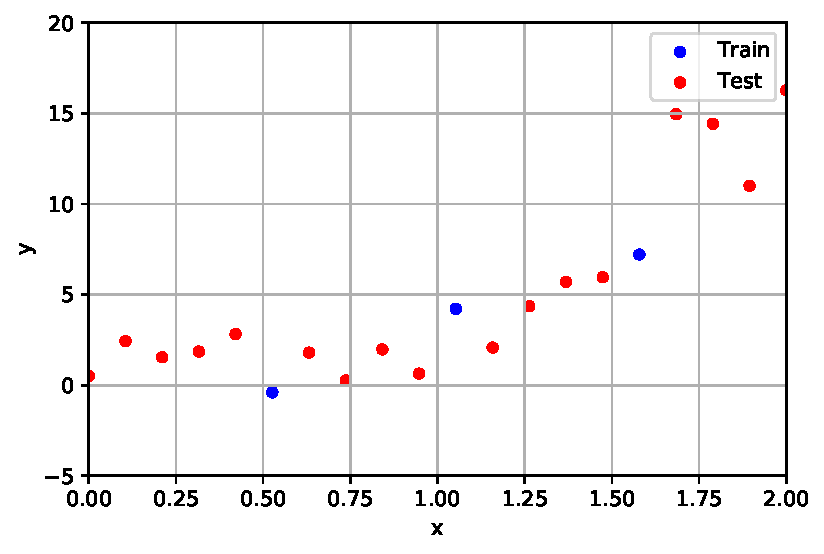
\includegraphics[width=0.85\linewidth]{figs/ex1_1_data.pdf}
		\caption{Scatterplot of train and test dataset}
		\label{fig:ex1_1_data}
	\end{figure}

	\subsection*{Error for different degree polynomials}
	
	In \prettyref{fig:ex1_1_mse_deg} the stemplot of the MSE over the test set is shown, the errors are logarithmically scaled. The smallest error is achieved for the degree $m=1$.
	
	\begin{figure}[H]
		\centering	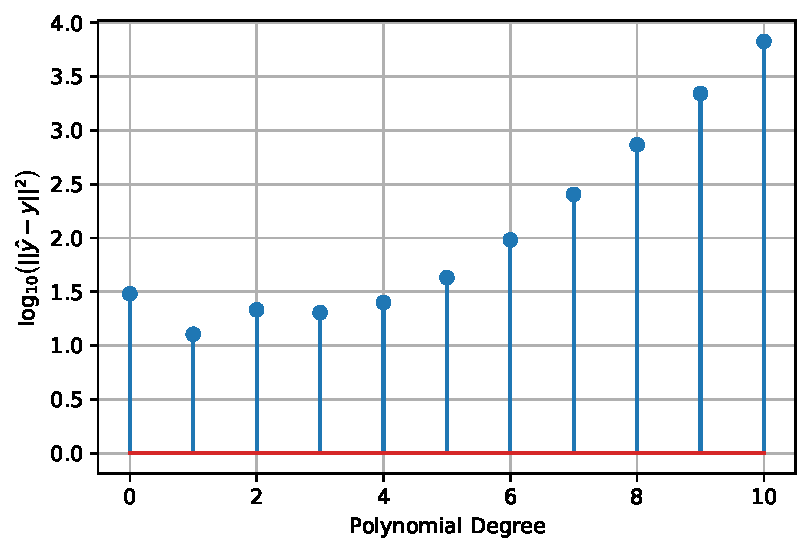
\includegraphics[width=0.85\linewidth]{figs/ex1_1_mse_degree.pdf}
		\caption{Stemplot showing the MSE for different degrees of the polynomial}
		\label{fig:ex1_1_mse_deg}
	\end{figure}

	\subsection*{Polynomial fit}
	
	In \prettyref{fig:ex1_1_poly_degrees} the polynomial fit is shown for different degrees on top of the two datasets. The value $m=1$ leads to the smallest error as was shown above. 
	For smaller values of $m$ the regressor is to simple (underfitting). The train set contains only three points, therefore for polynomials of degree $m\geq2$ the points in the train set can be captured exactly. Higher degree polynomials lead to very steep behaviour for $x > 1.5$, where there are no train datapoints anymore. Therefore the regressor generalizes poorly and has high error on the test set.
	So for $m \geq 2$ there is overfitting.
	
	\begin{figure}[H]
		\centering	
		\subfloat[][$m=0$]{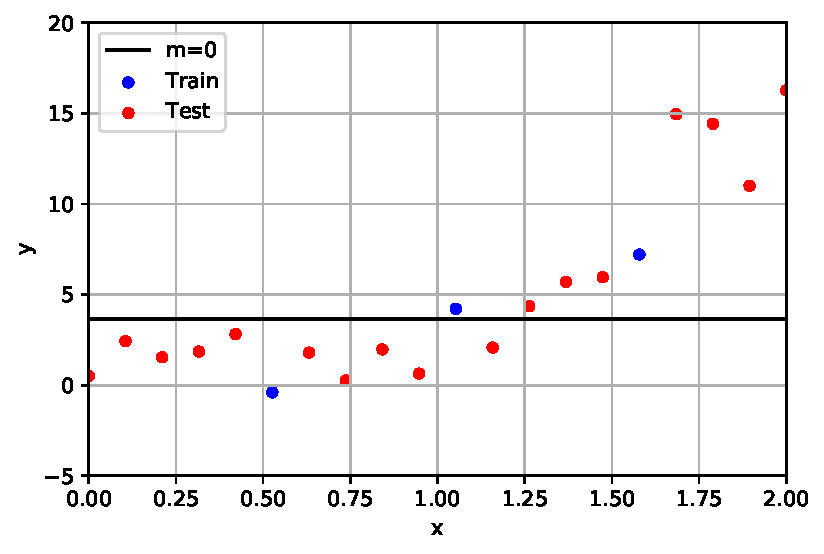
\includegraphics[width=0.3\linewidth]{figs/ex1_1_m0.pdf}}
		\subfloat[][$m=1$]{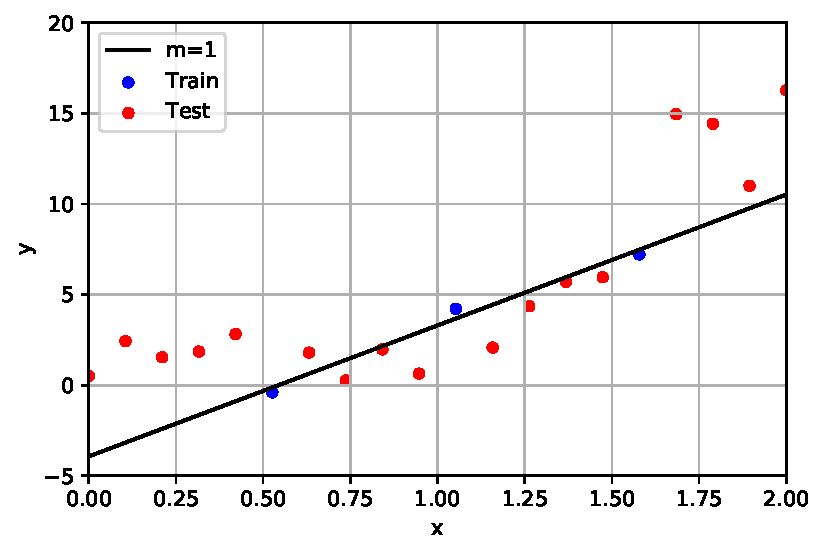
\includegraphics[width=0.3\linewidth]{figs/ex1_1_m1.pdf}}
		\subfloat[][$m=2$]{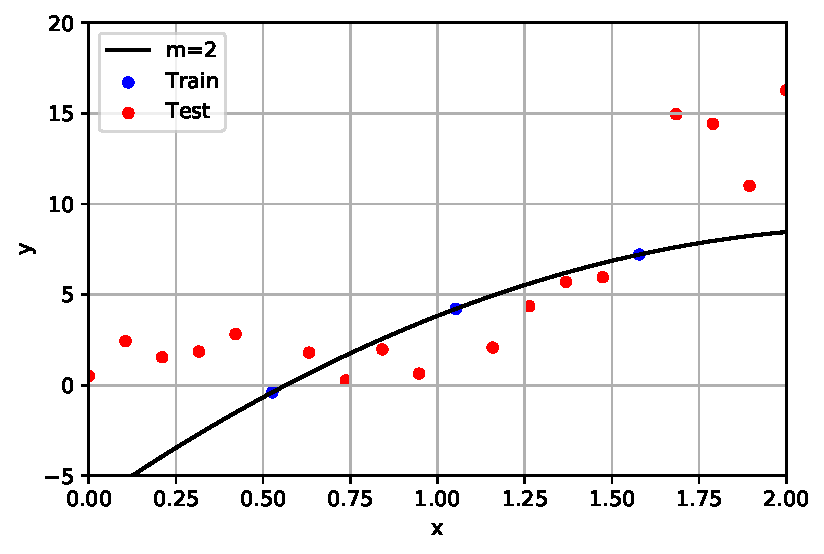
\includegraphics[width=0.3\linewidth]{figs/ex1_1_m2.pdf}}\\
		\subfloat[][$m=3$]{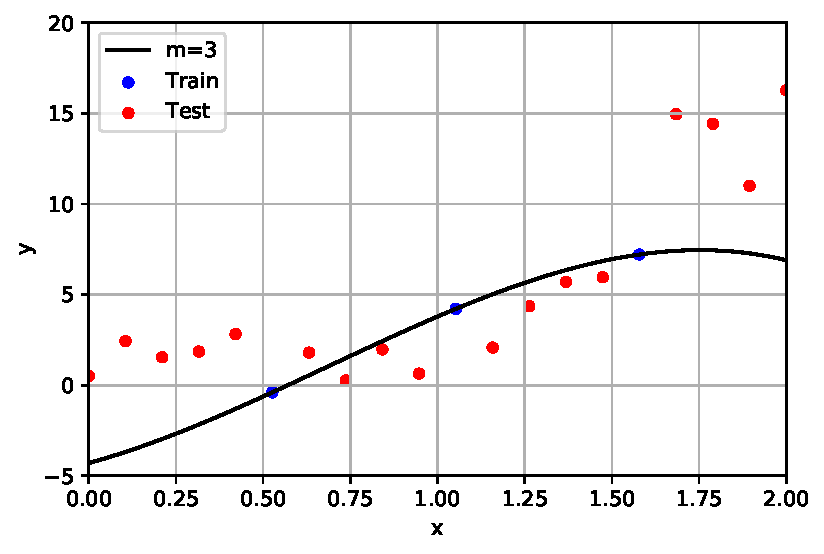
\includegraphics[width=0.3\linewidth]{figs/ex1_1_m3.pdf}}
		\subfloat[][$m=4$]{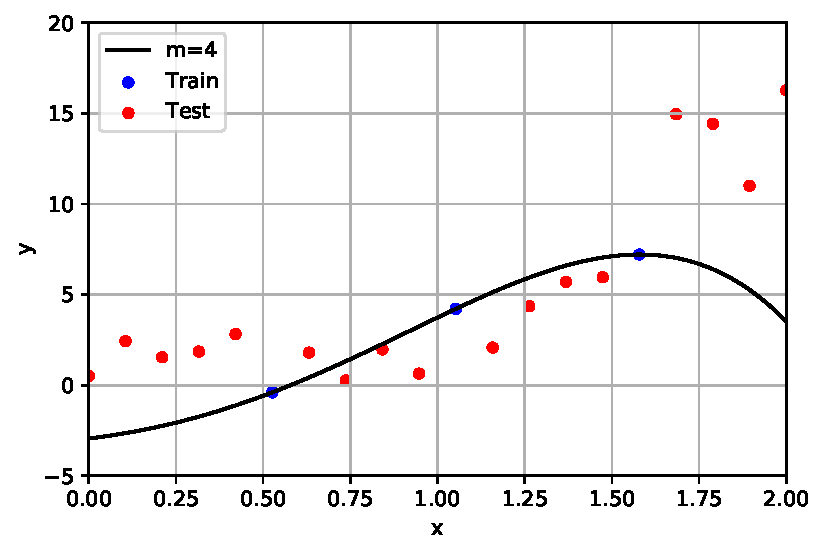
\includegraphics[width=0.3\linewidth]{figs/ex1_1_m4.pdf}}
		\subfloat[][$m=5$]{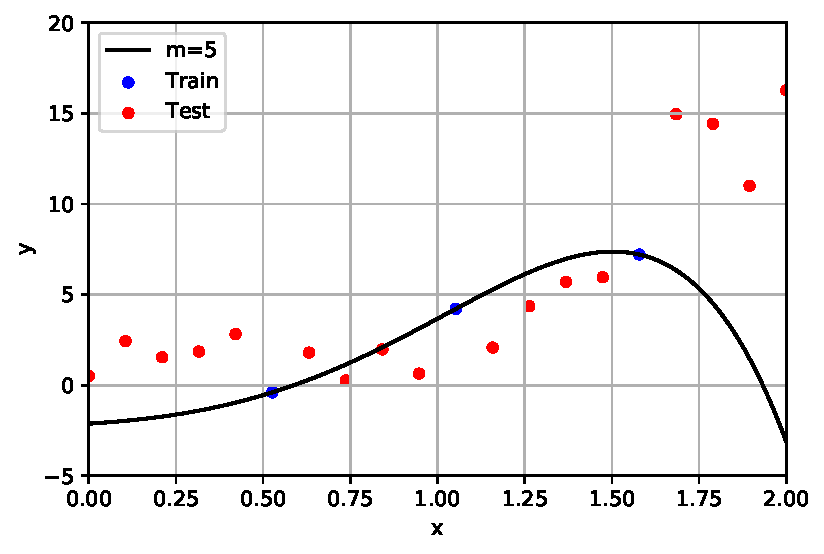
\includegraphics[width=0.3\linewidth]{figs/ex1_1_m5.pdf}}\\
		\subfloat[][$m=6$]{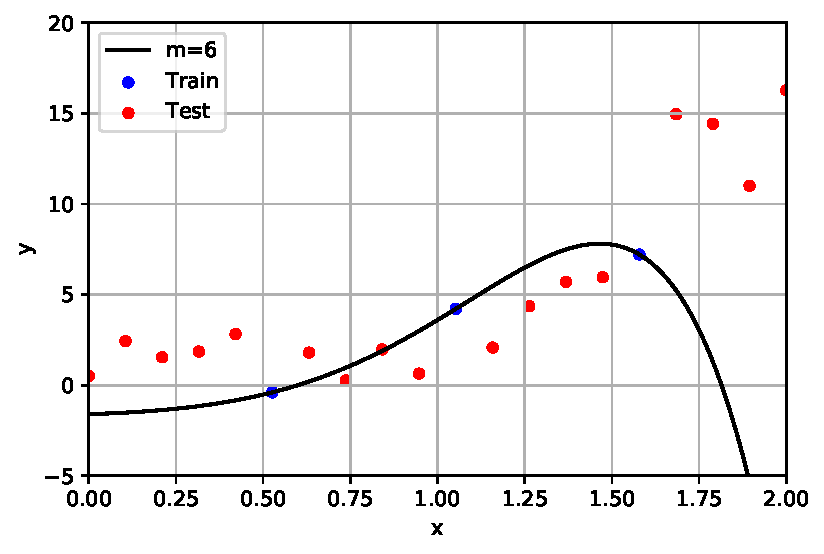
\includegraphics[width=0.3\linewidth]{figs/ex1_1_m6.pdf}}
		\subfloat[][$m=7$]{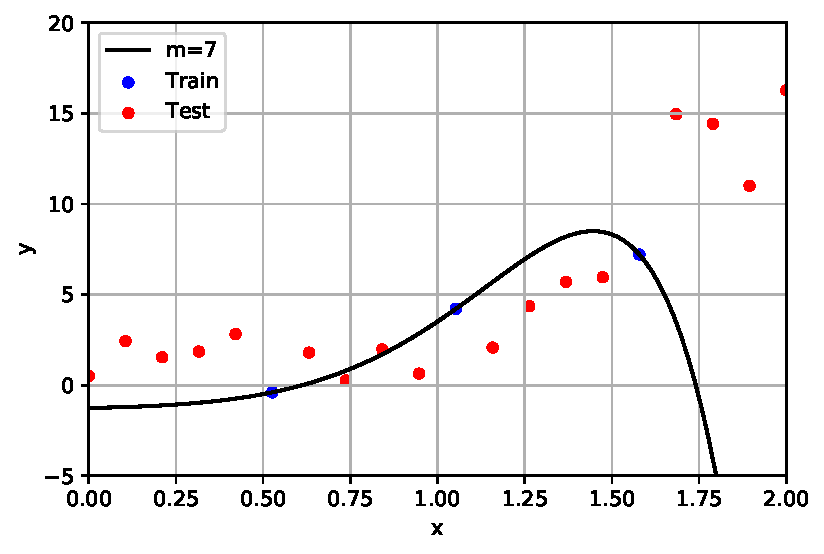
\includegraphics[width=0.3\linewidth]{figs/ex1_1_m7.pdf}}
		\subfloat[][$m=8$]{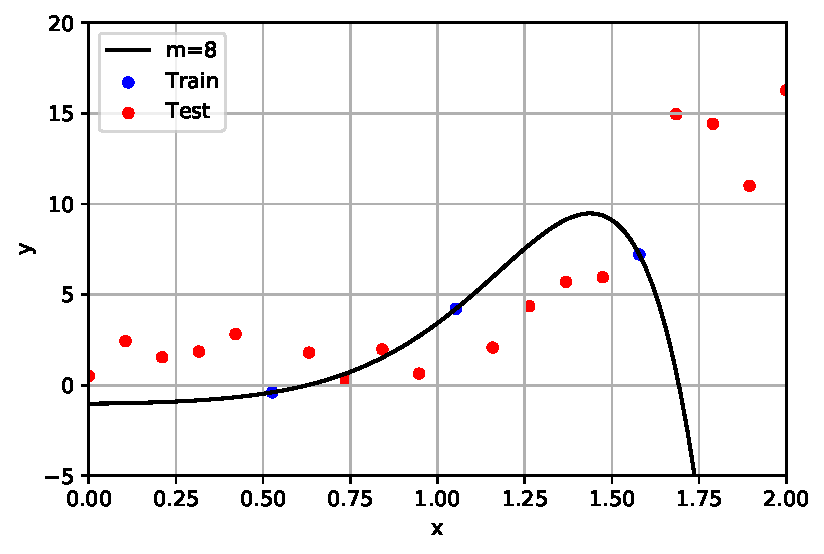
\includegraphics[width=0.3\linewidth]{figs/ex1_1_m8.pdf}}\\
		\subfloat[][$m=9$]{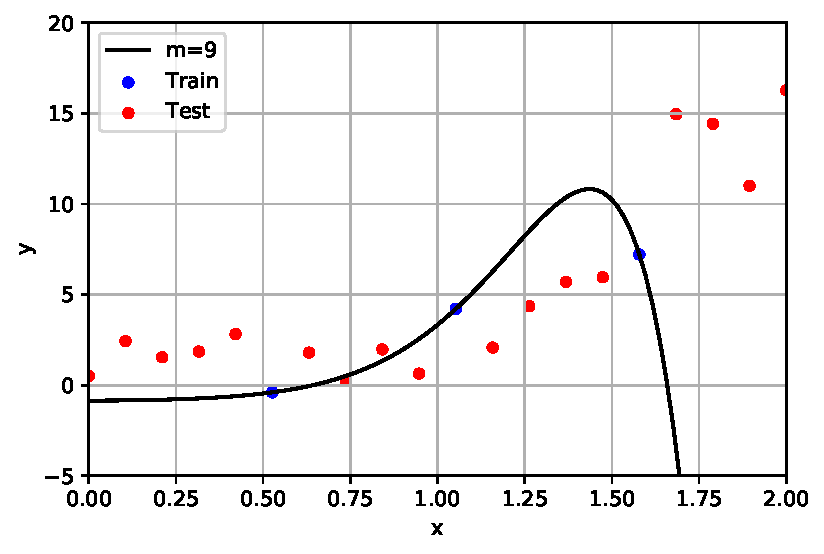
\includegraphics[width=0.3\linewidth]{figs/ex1_1_m9.pdf}}
		\subfloat[][$m=10$]{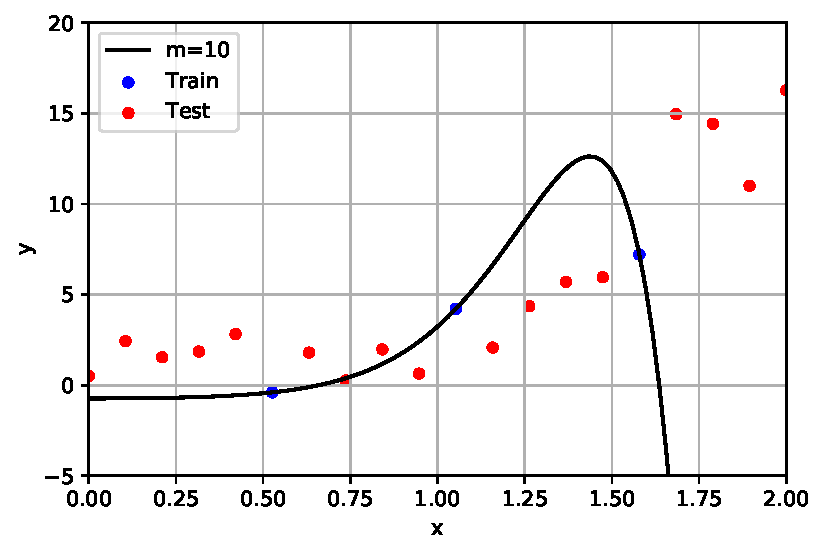
\includegraphics[width=0.3\linewidth]{figs/ex1_1_m10.pdf}}
		\caption{Polynomial fit for various different degrees $m$ of polynomial}
		\label{fig:ex1_1_poly_degrees}
	\end{figure}
	
	\subsection*{Ridge Regression Analytical}
	Cost function to be minimized
	\begin{equation}
		J(\matr{w}) = ||\matr{X}\matr{w}-\matr{y}||^2+\lambda ||\matr{w}||^2 = (\matr{X}\matr{w}-\matr{y})^T(\matr{X}\matr{w}-\matr{y})+\lambda\matr{w}^T\matr{w}
	\end{equation}
	
	with the matrix calculus rules given in the problem set:
	\begin{equation}
		\frac{\partial J\left( \matr{w}\right)}{\partial \matr{w}} = -2\matr{X}^T\matr{y}+2\matr{X}^T\matr{X}\matr{w}+2\lambda\matr{w}
	\end{equation}

	by setting the derivative to zero the optimal solution $\hat{\matr{w}}$ can be obtained.
	\begin{equation}
		\matr{X}^T\matr{X}\matr{w} + \lambda \matr{w} = \matr{X}^T\matr{y} \implies \hat{\matr{w}} = (\matr{X}^T\matr{X} + \lambda \matr{I})^{-1} \matr{X}^T\matr{y}
	\end{equation}
	
	\subsection*{Ridge Regression Errors}
	
	The errors over the test set for different values of $\lambda$ are shown in a log-log-plot in \prettyref{fig:ex1_1_mse_lambda}. The smallest error is achieved for $\lambda = 5$.
	
	
	\begin{figure}[H]
		\centering	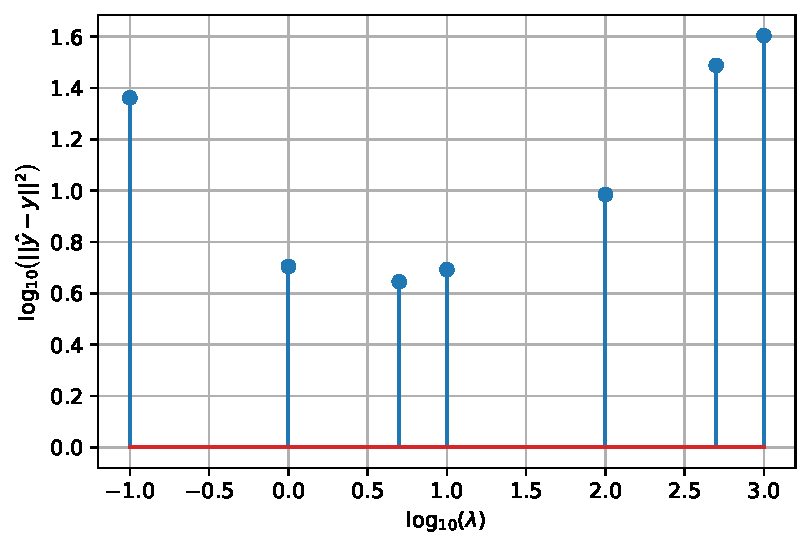
\includegraphics[width=0.85\linewidth]{figs/ex1_1_mse_lambda.pdf}
		\caption{Stemplot showing the MSE for different values of $\lambda$}
		\label{fig:ex1_1_mse_lambda}
	\end{figure}
	
	\subsection*{Ridge regression fit}
	
	For low values of $\lambda$ ($0$ or $0.1$) no regularizing effect is visible yet.
	The values $1.0$ and $5.0$ and $10.0$  deliver relatively good results with small error. For higher values of $\lambda$ the norm of $\matr{w}$ gets penalized more and more which forces the weights to become very small and therefore forces the polynomial towards zero. The error becomes higher for too high values of $\lambda$.
	A correct setting of $\lambda$ can prevent overfitting.
	
	
	\begin{figure}[H]
		\centering	
		\subfloat[][$\lambda=0$]{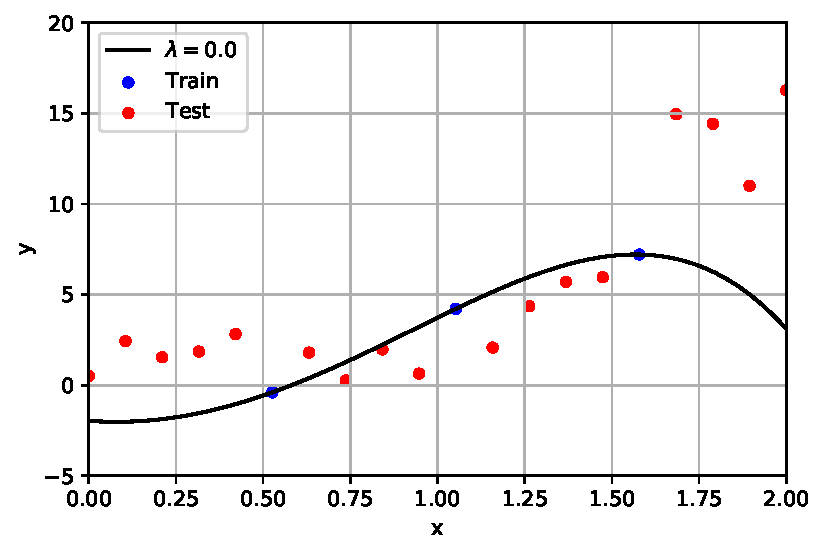
\includegraphics[width=0.3\linewidth]{figs/ex1_1_lamb0.pdf}}
		\subfloat[][$\lambda=0.1$]{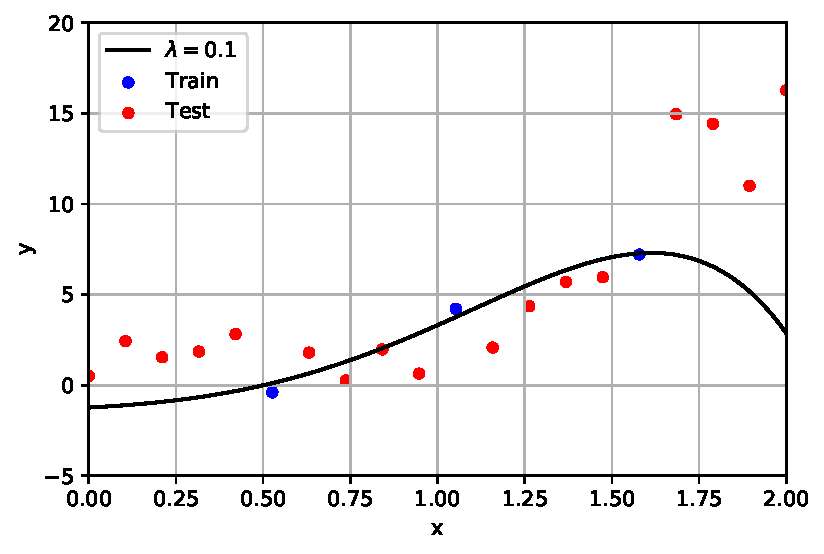
\includegraphics[width=0.3\linewidth]{figs/ex1_1_lamb1.pdf}}
		\subfloat[][$\lambda=1.0$]{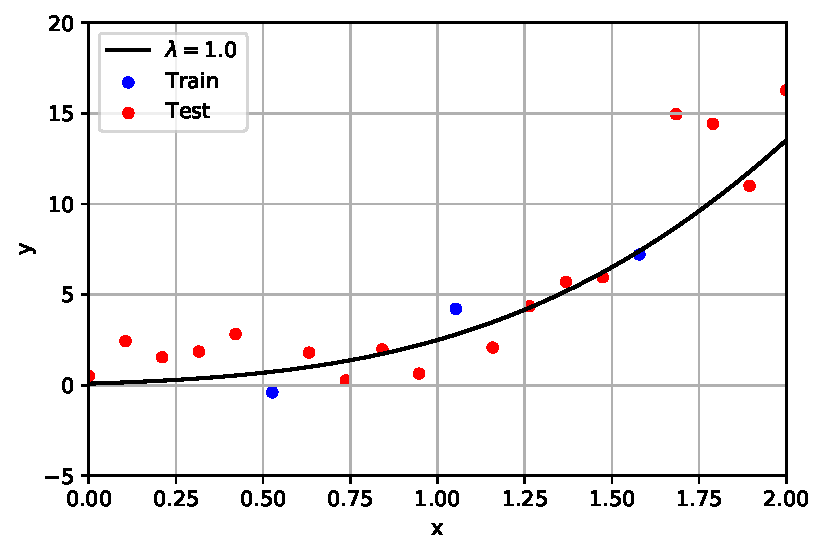
\includegraphics[width=0.3\linewidth]{figs/ex1_1_lamb2.pdf}}\\
		\subfloat[][$\lambda=5.0$]{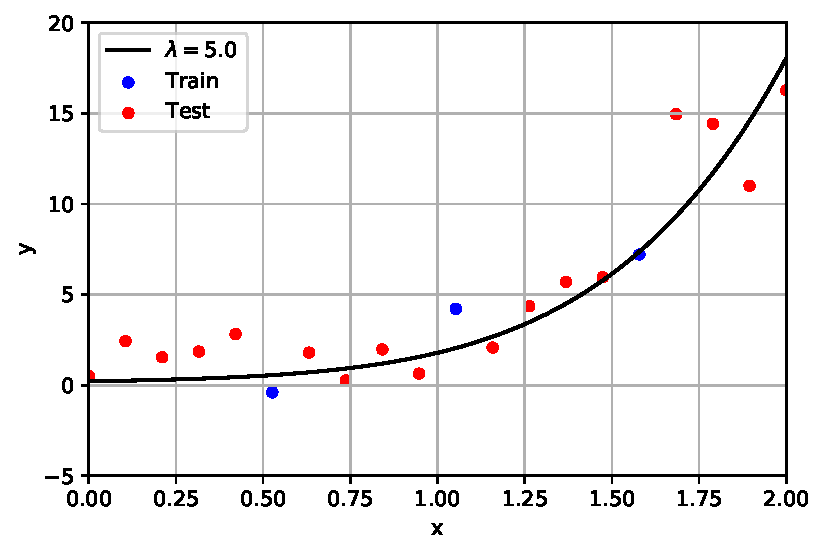
\includegraphics[width=0.3\linewidth]{figs/ex1_1_lamb3.pdf}}
		\subfloat[][$\lambda=10.0$]{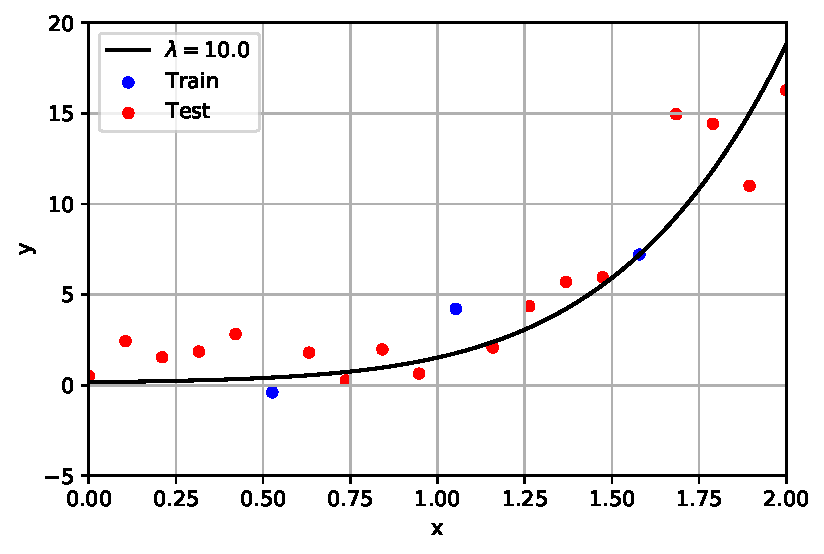
\includegraphics[width=0.3\linewidth]{figs/ex1_1_lamb4.pdf}}
		\subfloat[][$\lambda=100$]{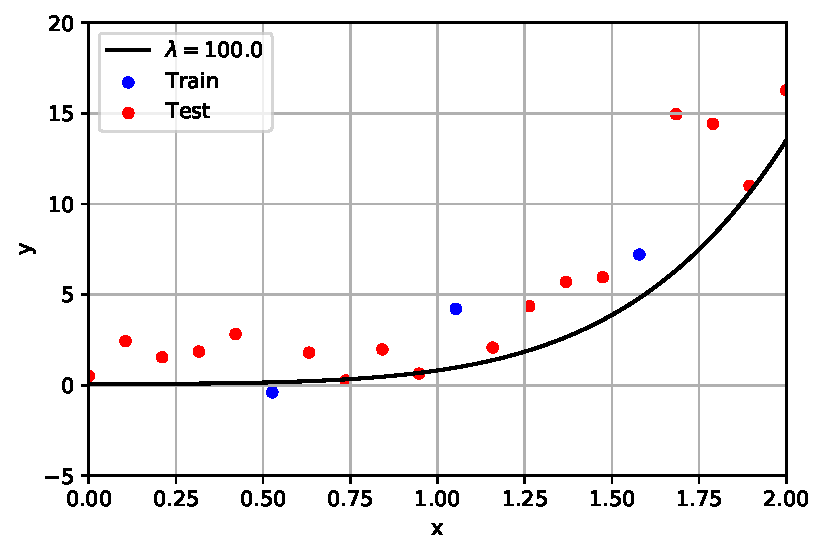
\includegraphics[width=0.3\linewidth]{figs/ex1_1_lamb5.pdf}}\\
		\subfloat[][$\lambda=500$]{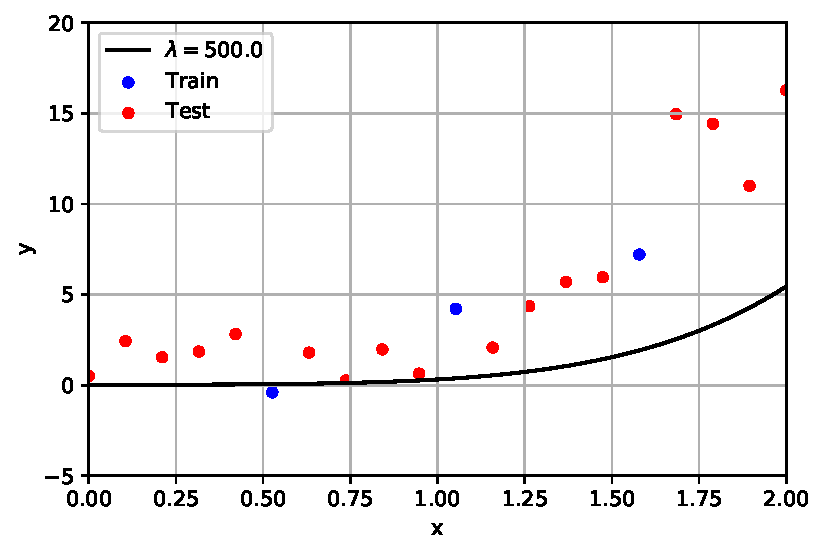
\includegraphics[width=0.3\linewidth]{figs/ex1_1_lamb6.pdf}}
		\subfloat[][$\lambda=1000$]{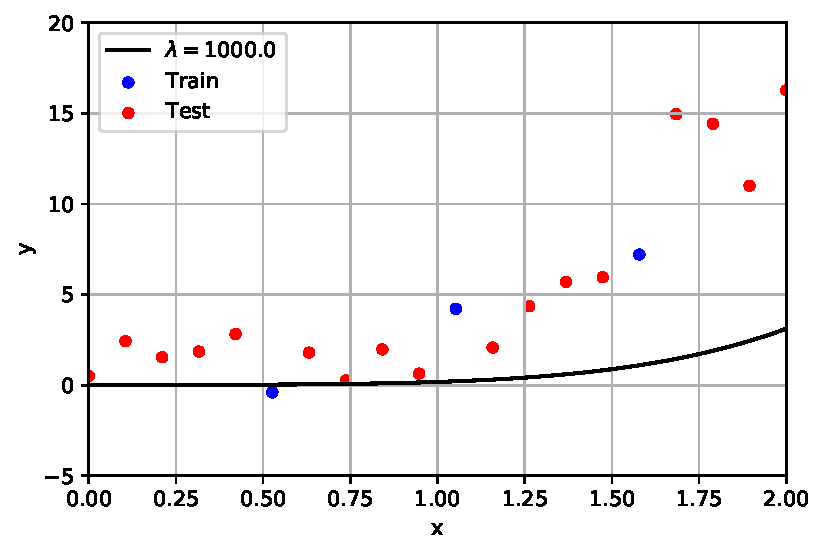
\includegraphics[width=0.3\linewidth]{figs/ex1_1_lamb7.pdf}}
		\caption{Ridge regressor fit for various different values of $\lambda$}
		\label{fig:ex1_1_lambda}
	\end{figure}
	
	 \section*{Problem 1.2}
	 \subsection*{Dataset}
	 The two datasets blob and moon are shown in \prettyref{fig:ex1_2_data_blob} and \prettyref{fig:ex1_2_data_moon}. For each dataset the train and test set are shown separately  and the two labels $\{-1, 1\}$ are shown in different colours.

	\begin{figure}[H]
		\centering	
		\subfloat[][Train Data]{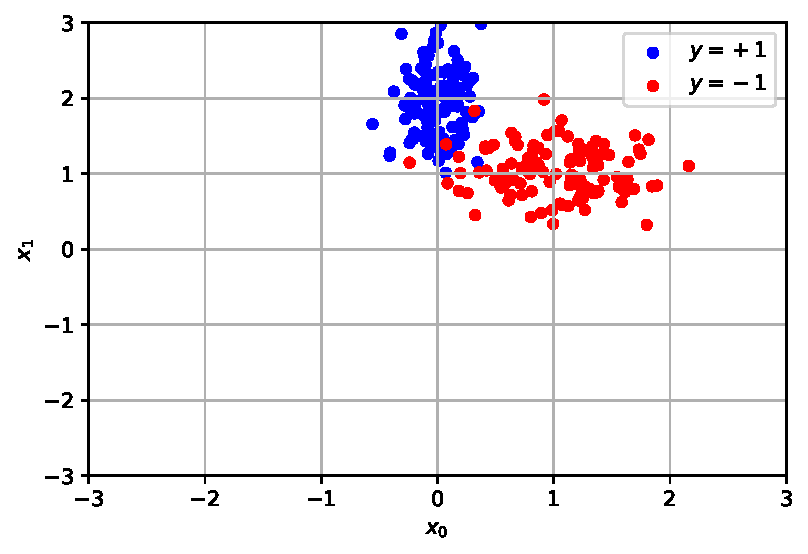
\includegraphics[width=0.45\linewidth]{figs/ex1_2_train_blob.pdf}}
		\subfloat[][Test Data]{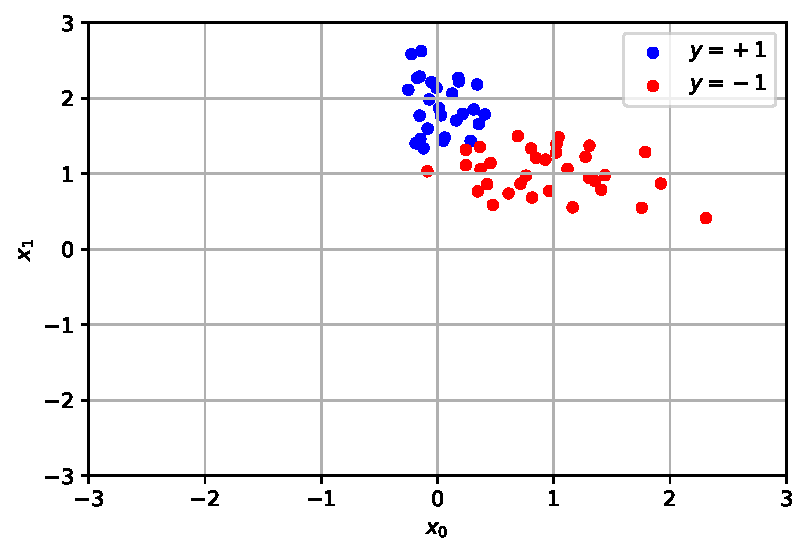
\includegraphics[width=0.45\linewidth]{figs/ex1_2_test_blob.pdf}}
		\caption{Scatterplot of train and test dataset blob}
		\label{fig:ex1_2_data_blob}
	\end{figure}

	\begin{figure}[H]
		\centering	
		\subfloat[][Train Data]{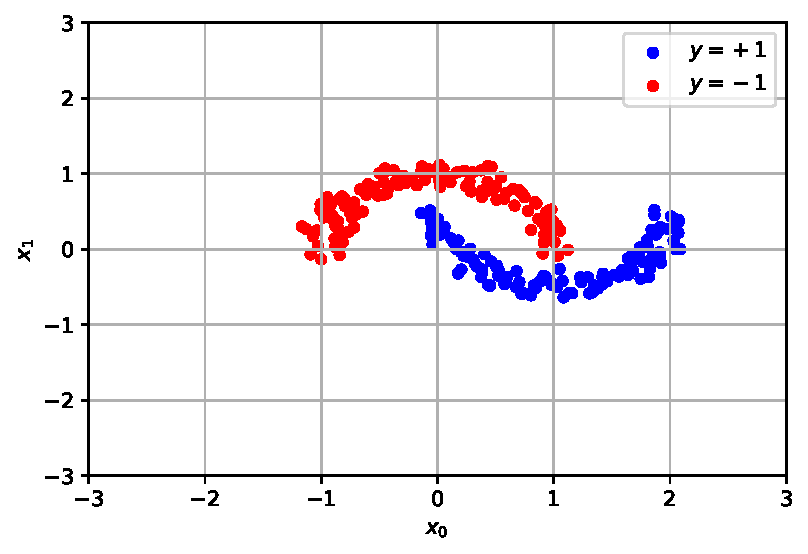
\includegraphics[width=0.45\linewidth]{figs/ex1_2_train_moon.pdf}}
		\subfloat[][Test Data]{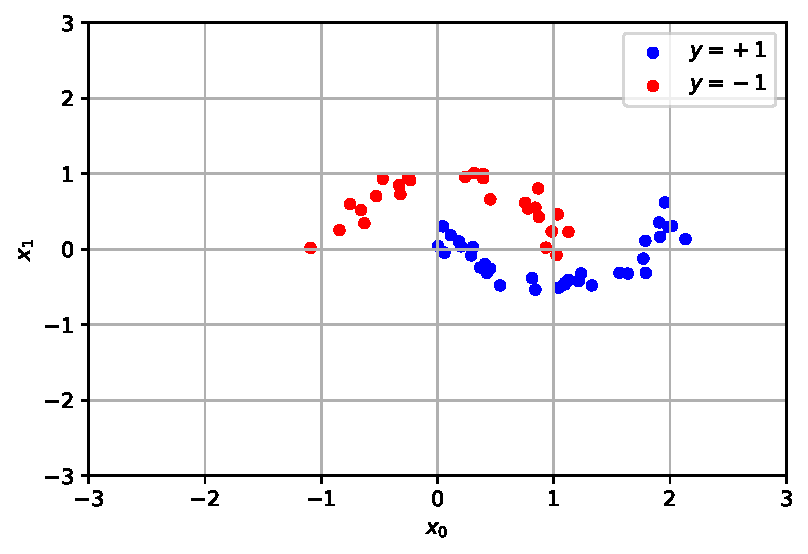
\includegraphics[width=0.45\linewidth]{figs/ex1_2_test_moon.pdf}}
		\caption{Scatterplot of train and test dataset moon}
		\label{fig:ex1_2_data_moon}
	\end{figure}
	 
	 \subsection*{Accuracy linear classifier}
	 
	 The accuracy of the linear classifier for the two datasets are shown in \prettyref{tab:ex1_2_accuracy_blob} and \prettyref{tab:ex1_2_accuracy_moon}. For both, the accuracy is shown on the train and test set separately.
	 
	 The accuracy for the moon dataset is worse because a linear classifier is not an optimal choice for this dataset as can be seen in the scatterplot.
	 
	 
	\begin{table}[H]
		\centering
		\begin{tabular}{|l|c|}
			\hline
			Train Accuracy & 97.92\% \\ \hline
			Test Accuracy  & 95.00\% \\ \hline
		\end{tabular}
		\caption{Accuracy of the linear classifier for blob dataset}
		\label{tab:ex1_2_accuracy_blob}
	\end{table}

	\begin{table}[H]
		\centering
		\begin{tabular}{|l|c|}
			\hline
			Train Accuracy & 87.08\% \\ \hline
			Test Accuracy  & 88.33\% \\ \hline
		\end{tabular}
		\caption{Accuracy of the linear classifier for moon dataset}
		\label{tab:ex1_2_accuracy_moon}
	\end{table}
	
	\subsection*{Heatmap}
	
	A heatmap of the soft-label output is shown in \prettyref{fig:ex1_2_heatmap_blob} and \prettyref{fig:ex1_2_heatmap_moon} for the two datasets.
	
	\begin{figure}[H]
		\centering	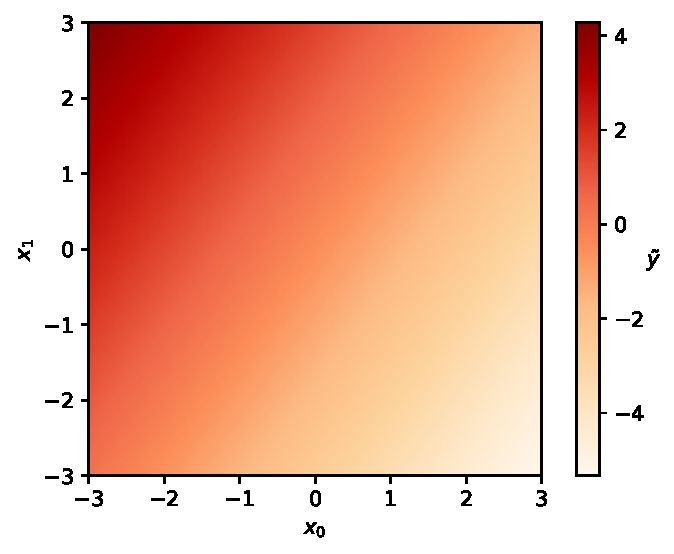
\includegraphics[width=0.5\linewidth]{figs/ex1_2_heatm_blob.pdf}
		\caption{Heatmap blob dataset}
		\label{fig:ex1_2_heatmap_blob}
	\end{figure}

	\begin{figure}[H]
		\centering	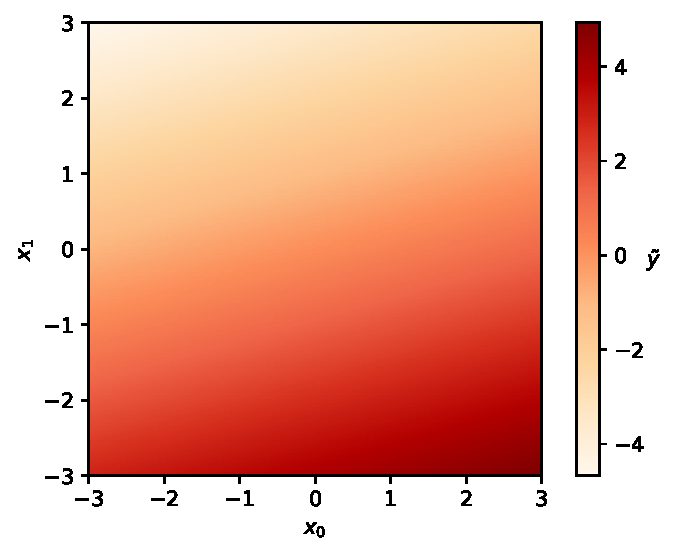
\includegraphics[width=0.5\linewidth]{figs/ex1_2_heatm_moon.pdf}
		\caption{Heatmap moon dataset}
		\label{fig:ex1_2_heatmap_moon}
	\end{figure}
	
	\subsection*{Decision Boundary}
	
	The decision boundary separating the two classes for the blob dataset is shown in \prettyref{fig:ex1_2_boundary_blob}.
	For the moon dataset it is shown in \prettyref{fig:ex1_2_boundary_moon}.
	As can be clearly seen, this dataset consists of two interleaving half circles. Therefore, a linear classifier is not the appropriate choice for this dataset. To better separate the two classes an S-shaped decision boundary would be needed, which cannot be achieved by a linear classifier.
	
	\begin{figure}[H]
		\centering	
		\subfloat[][Train]{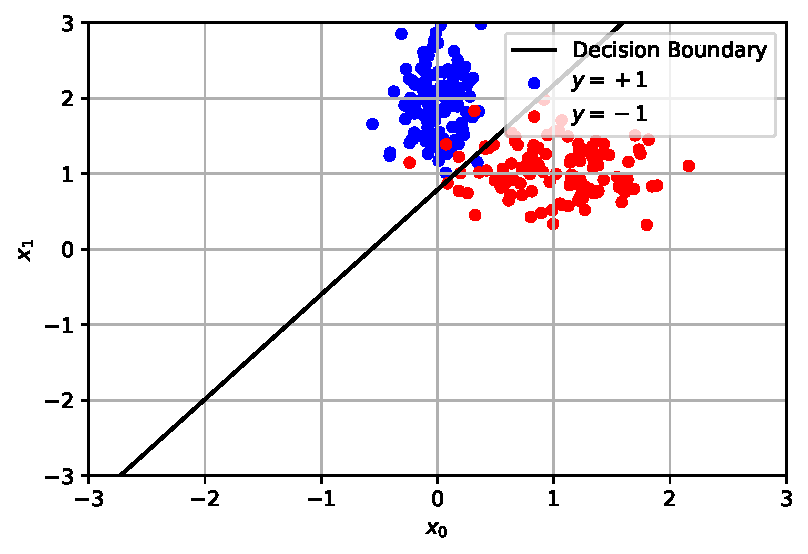
\includegraphics[width=0.45\linewidth]{figs/ex1_2_b_train_blob.pdf}}
		\subfloat[][Test]{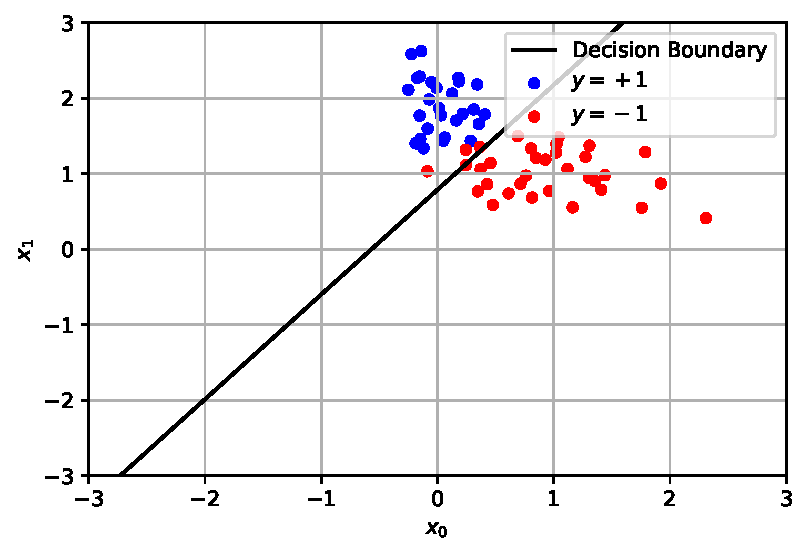
\includegraphics[width=0.45\linewidth]{figs/ex1_2_b_test_blob.pdf}}
		\caption{Scatterplot with decision Boundary}
		\label{fig:ex1_2_boundary_blob}
	\end{figure}

	\begin{figure}[H]
		\centering	
		\subfloat[][Train]{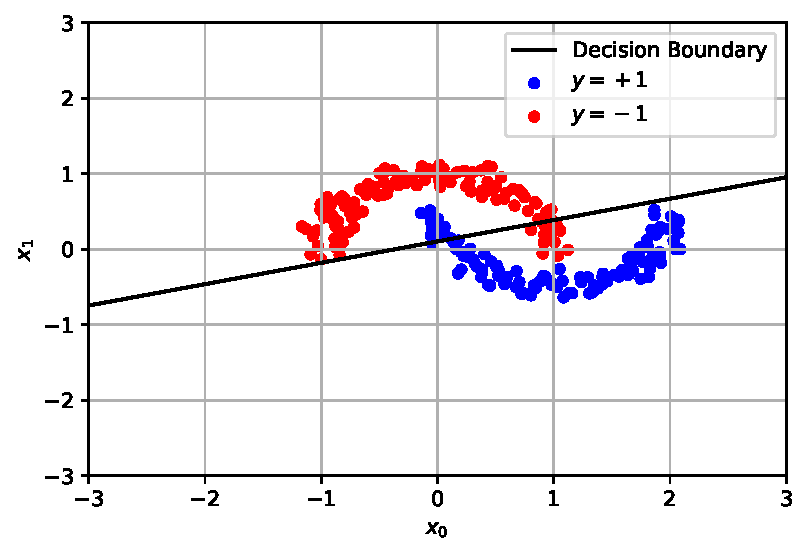
\includegraphics[width=0.45\linewidth]{figs/ex1_2_b_train_moon.pdf}}
		\subfloat[][Test]{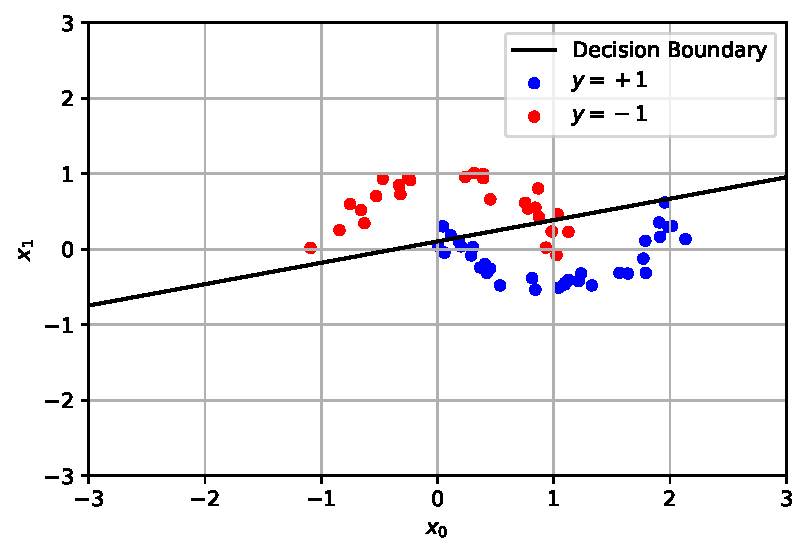
\includegraphics[width=0.45\linewidth]{figs/ex1_2_b_test_moon.pdf}}
		\caption{Scatterplot with decision Boundary moon dataset}
		\label{fig:ex1_2_boundary_moon}
	\end{figure}

	\subsection*{Loss comparison soft and hard labels}
	
	For the training of the classifier the MSE on the soft-labels has been chosen as loss function.
	For the two samples
	$s_1=\{[-10,10]^T, 1\}; s_2=\{[0, 1.5]^T, -1\}$ the loss is shown in \prettyref{tab:ex1_2_losses_blob}. 
	
	The sample $s_1$ has a loss value of $209.6$ even though as can be seen from the hard-label loss, the sample is correctly classified.
	The sample $s_2$ has a loss of only $2.180$ but is classified wrongly. 
	
	
	This indicates, that the MSE on the soft-labels is not ideal as loss function. A sample that is correctly classified but has a higher distance form the decision boundary contributes more the the loss function, than a sample that is close to the boundary and is classified wrongly.
	
	\begin{table}[H]
		\centering
		\begin{tabular}{ll|c|}
			\cline{3-3}
			&            & $J_\mathrm{LS}$ \\ \hline
			\multicolumn{1}{|l|}{\multirow{2}{*}{$s_1$}} & Soft Label & 209.6           \\ \cline{2-3} 
			\multicolumn{1}{|l|}{}                       & Hard Label & 0               \\ \hline
			\multicolumn{1}{|l|}{\multirow{2}{*}{$s_2$}} & Soft Label & 2.180           \\ \cline{2-3} 
			\multicolumn{1}{|l|}{}                       & Hard Label & 4               \\ \hline
		\end{tabular}
		\caption{Loss comparison of soft and hard labels for the two samples $s_1$ and $s_2$}
		\label{tab:ex1_2_losses_blob}
	\end{table}

	\section*{Problem 1.3}
	\subsection*{Dataset}
	
	As a quick sanity check, the correlation of the features with the median house value was computed. The values are reported in \prettyref{tab:ex1_3_corr}. The feature MedInc has the highest correlation with the target value.	
	
	\begin{table}[H]
		\centering
		\begin{tabular}{|l|c|}
			\hline
			MedInc     & $\num{0.688075}$  \\ \hline
			AveRooms   & $\num{0.151948}$  \\ \hline
			HouseAge   & $\num{0.105623}$  \\ \hline
			AveOccup   & $\num{-0.023737}$ \\ \hline
			Population & $\num{-0.024650}$ \\ \hline
			Longitude  & $\num{-0.045967}$ \\ \hline
			AveBedrms  & $\num{-0.046701}$ \\ \hline
			Latitude   & $\num{-0.144160}$ \\ \hline
		\end{tabular}
		\caption{Correlation with MedHouseVal sorted highest to lowest}
		\label{tab:ex1_3_corr}
	\end{table}

	
	
	\subsection*{Scatterplot of Median House Value}
	
	A scatterplot of the datapoints in a longitude latitude diagram is shown in \prettyref{fig:ex1_3_scatter_lon_lat}, the color indicates the target value.
	The data outlines California and it can be seen that along the coast and near the large cities the target value is higher, further the density of data points is higher in those areas.
	
	\begin{figure}[H]
		\centering	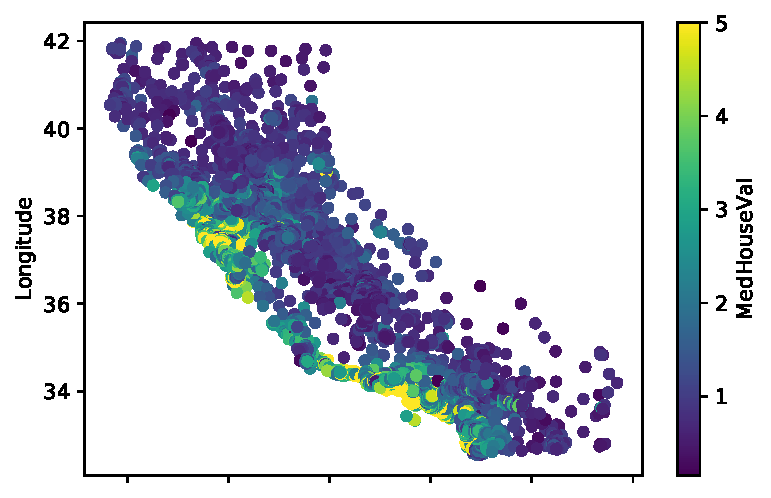
\includegraphics[width=0.5\linewidth]{figs/ex1_3_lon_lat.pdf}
		\caption{scatterplot longitude lattitude}
		\label{fig:ex1_3_scatter_lon_lat}
	\end{figure}
	
	
	In \prettyref{fig:ex1_3_hist_lon_lat} a histogram of longitude and latitude is shown.
	The two highest peaks are at approximately $-122$ and $-118.2$ for longitude and $34$ and $37.8$ for latitude.
	The four most populous cities in California are listed in \prettyref{tab:ex1_3_coords_cal}. The cities Los Angeles and San Jose / San Francisco match up very good with the two highest peaks in the histograms.
	
	\begin{table}[H]
		\centering
		\begin{tabular}{|l|r|r|} \hline
			City & Longitude & Latitude \\ \hline
			Los Angeles & -118.24 & 34.05 \\ \hline
			San Diego & -117.16 & 32.72 \\ \hline
			San Jose & -121.89 & 37.34 \\ \hline
			San Francisco & -122.42 & 37.77 \\ \hline
		\end{tabular}
		\caption{Coordinates of the four most populous cities in California}
		\label{tab:ex1_3_coords_cal}
	\end{table}


	\begin{figure}[H]
		\centering	
		\subfloat[][Longitude]{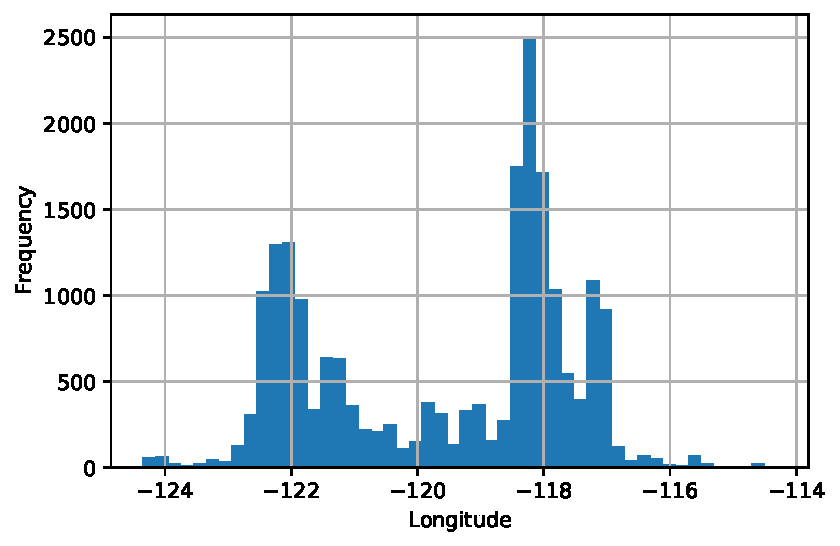
\includegraphics[width=0.45\linewidth]{figs/ex1_3_hist_lon.pdf}}
		\subfloat[][Latitude]{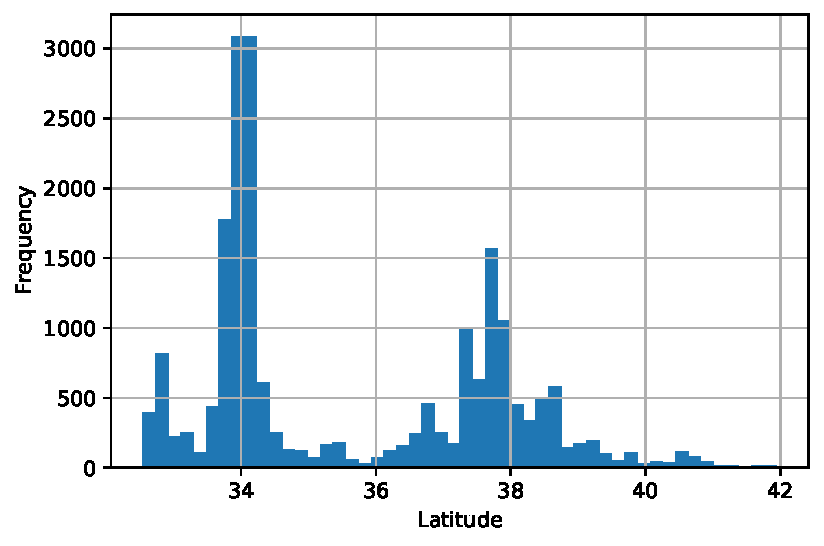
\includegraphics[width=0.45\linewidth]{figs/ex1_3_hist_lat.pdf}}
		\caption{Histograms of longitude and latitude}
		\label{fig:ex1_3_hist_lon_lat}
	\end{figure}
	
	\subsection*{Weights of Ridge Regressor}
	
	In \prettyref{tab:ex1_3_weights} the weights for the ridge regressor are shown. In \prettyref{tab:ex1_3_intercept} the intercept can be seen.
	The Features AveBedrms, MedInc, HouseAge have a positive impact on the house price, all the other features have negativ impact on the house price.
	
	The intercept is very high, as for example the Longitude and Latitude have an Offset, those values are not centered around zero.
	
	
	\begin{table}[H]
		\centering
		\begin{tabular}{|l|c|}
			\hline
			Feature    & Weight            \\ \hline
			AveBedrms  & $\num{8.16e-1}$  \\ \hline
			MedInc     & $\num{4.48e-1}$  \\ \hline
			HouseAge   & $\num{9.59e-3}$  \\ \hline
			Population & $\num{-6.09e-7}$ \\ \hline
			AveOccup   & $\num{-4.63e-3}$ \\ \hline
			AveRooms   & $\num{-1.33e-1}$ \\ \hline
			Latitude   & $\num{-4.63e-1}$ \\ \hline
			Longitude  & $\num{-4.36e-1}$ \\ \hline
		\end{tabular}
		\caption{Features and corresponding weights of the ridge regressor sorted by the weights}
		\label{tab:ex1_3_weights}
	\end{table}
	
	\begin{table}[H]
		\centering
		\begin{tabular}{|l|c|} 
			\hline
			Intercept & $-37.3$  \\ \hline
		\end{tabular}
		\caption{Intercept of ridge regressor}
		\label{tab:ex1_3_intercept}
	\end{table}
	
	
	\subsection*{Comparison of regressors}
	
	In \prettyref{tab:ex1_3_mae} the mean average error has been computed on the train and test set for both regressors.
	
	The ridge regressor performs approximately equal on the train and the test dataset. 
	The random forest regressor has lower MAE on the train dataset than on the test dataset. This might indicate that the regressor is close to or already in an overfitting regime.
	Overall the random forest regressor performs better on the test set. This is to be expected because it can capture the more complex relationships in the data, which cannot be captured by a linear regressor.
	
	\begin{table}[H]
		\centering
		\begin{tabular}{ll|c|}
			\cline{3-3}
			&       & MAE   \\ \hline
			\multicolumn{1}{|l|}{\multirow{2}{*}{Ridge Regressor}}         & Train & 0.531 \\ \cline{2-3} 
			\multicolumn{1}{|l|}{}                                         & Test  & 0.528 \\ \hline
			\multicolumn{1}{|l|}{\multirow{2}{*}{Random Forest Regressor}} & Train & 0.125 \\ \cline{2-3} 
			\multicolumn{1}{|l|}{}                                         & Test  & 0.331 \\ \hline
		\end{tabular}
		\caption{Mean Average Errors}
		\label{tab:ex1_3_mae}
	\end{table}
	
	In \prettyref{fig:ex1_3_hist_lin_rf} a histogram of the prediction error $\hat{y}-y$ is shown for 
	the two regressors. For each a separate histogram is shown for the train and test set.
	The histograms of both regressors are approximately centered around zero, which indicates that both regressors are unbiased.
	The histogram of the random forest regressor is much narrower, the error variance is lower.
	
	
	\begin{figure}[H]
		\centering	
		\subfloat[][Ridge Train]{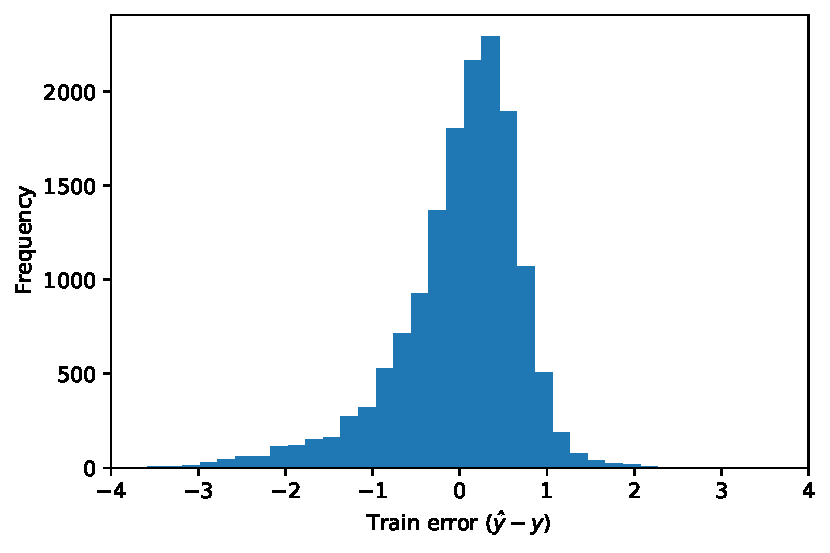
\includegraphics[width=0.45\linewidth]{figs/ex1_3_lin_hist_train.pdf}}
		\subfloat[][Random Forest Train]{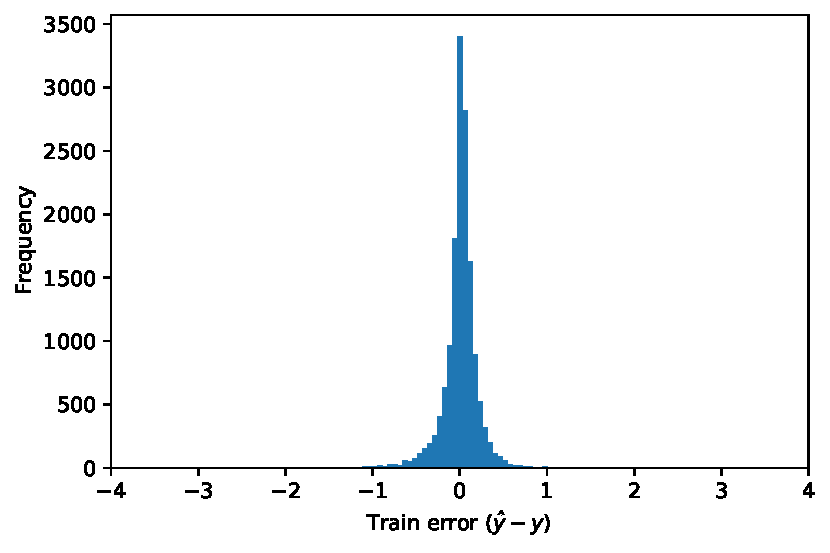
\includegraphics[width=0.45\linewidth]{figs/ex1_3_rf_hist_train.pdf}}\\
		\subfloat[][Ridge Test]{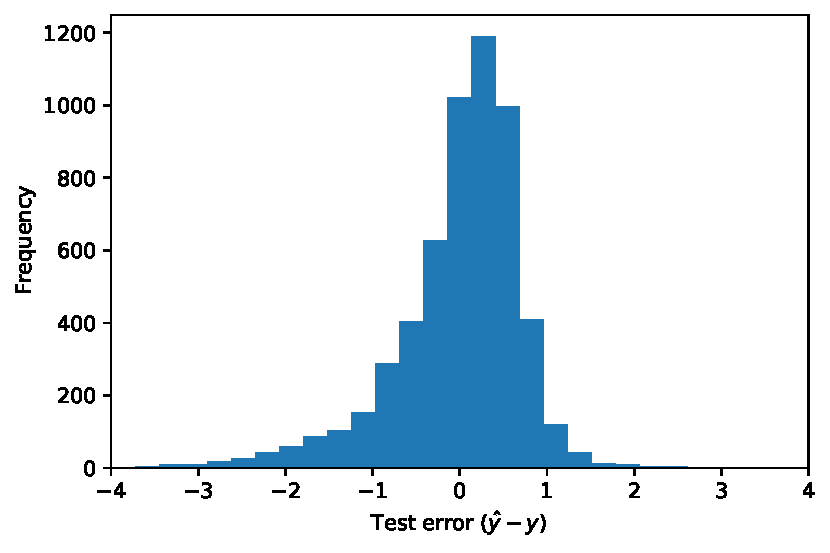
\includegraphics[width=0.45\linewidth]{figs/ex1_3_lin_hist_test.pdf}}
		\subfloat[][Random Forest Test]{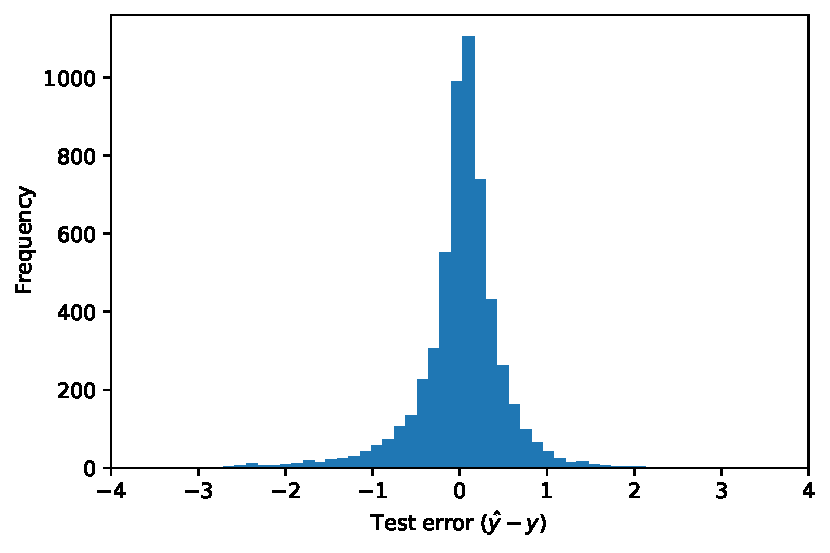
\includegraphics[width=0.45\linewidth]{figs/ex1_3_rf_hist_test.pdf}}
		\caption{Error histgrams for ridge regressor and random forest regressor}
		\label{fig:ex1_3_hist_lin_rf}
	\end{figure}
	

	In \prettyref{fig:ex1_3_scatter_lin_rf} the predicted over the actual values are shown for both regressors over the test set. Ideally alle data points would lie on a straight $ 45^ \circ $ line. It can be seen that the random forest regressor performs better because the points are closer to the ideal ones.
	
	\begin{figure}[H]
		\centering	
		\subfloat[][Ridge]{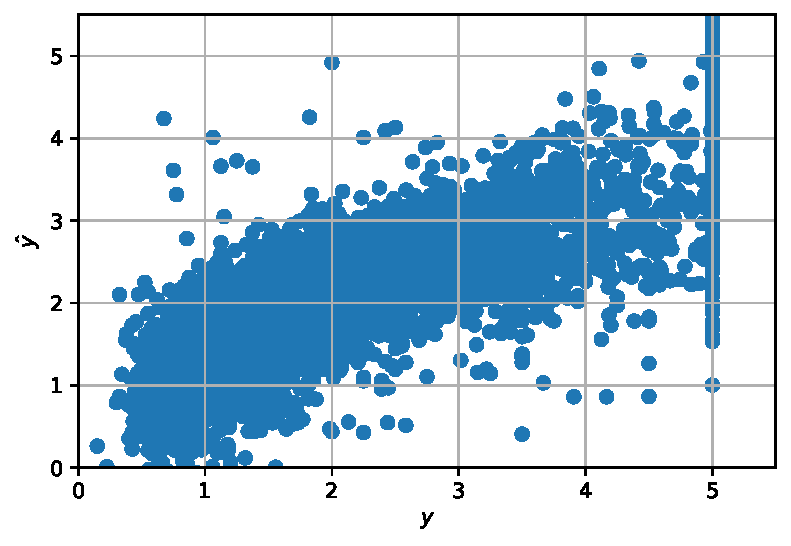
\includegraphics[width=0.45\linewidth]{figs/ex1_3_lin_scatter.pdf}}
		\subfloat[][Random Forest]{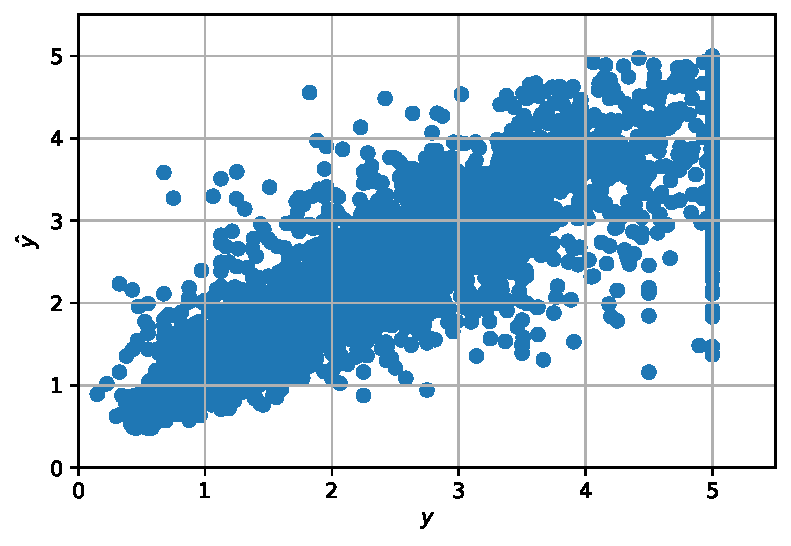
\includegraphics[width=0.45\linewidth]{figs/ex1_3_rf_scatter.pdf}}
		\caption{Scatter plot comparison of ridge regressor and random forest regressor over the test set}
		\label{fig:ex1_3_scatter_lin_rf}
	\end{figure}




	\subsection*{Cross Validation}
	
	The results of the 10-fold cross validation are reported in \prettyref{tab:ex1_3_cross_val}.
	The standard deviation is relatively low, indicating that the regressor performs comparable on all 10 splits of the cross validation.
	
	\begin{table}[H]
		\centering
		\begin{tabular}{|l|l|c|} \hline
			Mean               & 0.811  \\ \hline
			Standard deviation & 0.0097 \\ \hline
		\end{tabular}
		\caption{Mean and standard deviation of 10 fold cross-validation}
		\label{tab:ex1_3_cross_val}
	\end{table}

\end{document}